\documentclass[12pt,letterpaper]{article}
\usepackage{graphicx,textcomp}
\usepackage{natbib}
\usepackage{setspace}
\usepackage{fullpage}
\usepackage{color}
\usepackage[reqno]{amsmath}
\usepackage{amsthm}
\usepackage{fancyvrb}
\usepackage{amssymb,enumerate}
\usepackage[all]{xy}
\usepackage{endnotes}
\usepackage{lscape}
\newtheorem{com}{Comment}
\usepackage{float}
\usepackage{hyperref}
\newtheorem{lem} {Lemma}
\newtheorem{prop}{Proposition}
\newtheorem{thm}{Theorem}
\newtheorem{defn}{Definition}
\newtheorem{cor}{Corollary}
\newtheorem{obs}{Observation}
\usepackage[compact]{titlesec}
\usepackage{dcolumn}
\usepackage{tikz}
\usetikzlibrary{arrows}
\usepackage{multirow}
\usepackage{xcolor}
\newcolumntype{.}{D{.}{.}{-1}}
\newcolumntype{d}[1]{D{.}{.}{#1}}
\definecolor{light-gray}{gray}{0.65}
\usepackage{url}
\usepackage{listings}
\usepackage{color}

\definecolor{codegreen}{rgb}{0,0.6,0}
\definecolor{codegray}{rgb}{0.5,0.5,0.5}
\definecolor{codepurple}{rgb}{0.58,0,0.82}
\definecolor{backcolour}{rgb}{0.95,0.95,0.92}

\lstdefinestyle{mystyle}{
	backgroundcolor=\color{backcolour},   
	commentstyle=\color{codegreen},
	keywordstyle=\color{magenta},
	numberstyle=\tiny\color{codegray},
	stringstyle=\color{codepurple},
	basicstyle=\footnotesize,
	breakatwhitespace=false,         
	breaklines=true,                 
	captionpos=b,                    
	keepspaces=true,                 
	numbers=left,                    
	numbersep=5pt,                  
	showspaces=false,                
	showstringspaces=false,
	showtabs=false,                  
	tabsize=2
}
\lstset{style=mystyle}
\newcommand{\Sref}[1]{Section~\ref{#1}}
\newtheorem{hyp}{Hypothesis}

\title{Problem Set 1 Answers1}
\date{\today}
\author{Kaley Burg}


\begin{document}
	\maketitle
	\section*{Instructions}
	\begin{itemize}
	\item Please show your work! You may lose points by simply writing in the answer. If the problem requires you to execute commands in \texttt{R}, please include the code you used to get your answers. Please also include the \texttt{.R} file that contains your code. If you are not sure if work needs to be shown for a particular problem, please ask.
\item Your homework should be submitted electronically on GitHub in \texttt{.pdf} form.
\item This problem set is due before 23:59 on Sunday February 11, 2024. No late assignments will be accepted.
	\end{itemize}

	\vspace{.25cm}
\section*{Question 1} 
\vspace{.25cm}
\noindent The Kolmogorov-Smirnov test uses cumulative distribution statistics test the similarity of the empirical distribution of some observed data and a specified PDF, and serves as a goodness of fit test. The test statistic is created by:

$$D = \max_{i=1:n} \Big\{ \frac{i}{n}  - F_{(i)}, F_{(i)} - \frac{i-1}{n} \Big\}$$

\noindent where $F$ is the theoretical cumulative distribution of the distribution being tested and $F_{(i)}$ is the $i$th ordered value. Intuitively, the statistic takes the largest absolute difference between the two distribution functions across all $x$ values. Large values indicate dissimilarity and the rejection of the hypothesis that the empirical distribution matches the queried theoretical distribution. The p-value is calculated from the Kolmogorov-
Smirnoff CDF:

$$p(D \leq d)= \frac{\sqrt {2\pi}}{d} \sum _{k=1}^{\infty }e^{-(2k-1)^{2}\pi ^{2}/(8d^{2})}$$


\noindent which generally requires approximation methods (see \href{https://core.ac.uk/download/pdf/25787785.pdf}{Marsaglia, Tsang, and Wang 2003}). This so-called non-parametric test (this label comes from the fact that the distribution of the test statistic does not depend on the distribution of the data being tested) performs poorly in small samples, but works well in a simulation environment. Write an \texttt{R} function that implements this test where the reference distribution is normal. Using \texttt{R} generate 1,000 Cauchy random variables (\texttt{rcauchy(1000, location = 0, scale = 1)}) and perform the test (remember, use the same seed, something like \texttt{set.seed(123)}, whenever you're generating your own data).\\
	
	
\noindent As a hint, you can create the empirical distribution and theoretical CDF using this code:

\begin{lstlisting}[language=R]
	# create empirical distribution of observed data
	ECDF <- ecdf(data)
	empiricalCDF <- ECDF(data)
	# generate test statistic
	D <- max(abs(empiricalCDF - pnorm(data))) \end{lstlisting}

\textbf{My Answer:}

\begin{itemize}
	\item First I created my data 
	\lstinputlisting[language=R, firstline=42, lastline=42]{PS1_KB_Final.R}
	\lstinputlisting[language=R, firstline=46, lastline=46]{PS1_KB_Final.R}
	\item Then I created my Kolmogorov-Smirnoff CDF function:
	\lstinputlisting[language=R, firstline=53, lastline=89]{PS1_KB_Final.R}
	\item Lastly, I compared this with the built in ks.test function in R to check my answer
	\lstinputlisting[language=R, firstline=94, lastline=94]{PS1_KB_Final.R}
	\item The results of both my function and the ks.test output are shown in the tables below:


\begin{table}[!htbp] \centering 
	\caption{Kolmogorov-Smirnov Test - My function} 
	\label{tab:ks_output2} 
	\begin{tabular}{@{\extracolsep{5pt}}lc} 
		\\[-1.8ex]\hline 
		\hline \\[-1.8ex] 
		Statistic & Value \\ 
		\hline \\[-1.8ex] 
		$D$ & 0.1347281 \\ 
		$p$ & $5.652523 \times 10^{-29}$ \\ 
		\hline \\[-1.8ex] 
	\end{tabular} 
\end{table}

\begin{table}[!htbp] \centering 
	\caption{Kolmogorov-Smirnov Test - ks.test Output} 
	\label{tab:ks_output1} 
	\begin{tabular}{@{\extracolsep{5pt}}lc} 
		\\[-1.8ex]\hline 
		\hline \\[-1.8ex] 
		Statistic & Value \\ 
		\hline \\[-1.8ex] 
		D & 0.13573 \\ 
		$p$-value & $2.22 \times 10^{-16}$ \\ 
		\hline \\[-1.8ex] 
	\end{tabular} 
\end{table} 


\item Note: the results are slightly different between my function and ks.test due to internal differences in the function, but they are similar enough to show that my function was implemented correctly.
\newline \textbf{Interpretation:}
\item As stated above, the D statistic is the largest absolute difference between the two distributions across all x values. 
\item As shown in the tables above, the D statistic is approximately 0.13 and the p-value associated with this statistic is very close to 0.
\item This test overall assesses whether a sample comes from a specific distribution. Based on the p-statistic we obtain, we can draw the conclusion that we can \textbf{reject the null hypothesis that the sample is drawn from the reference (normal) distribution}. This value would be significant at the $\alpha <$ 0.001 level, due to how small the obtained p-statistic is


\end{itemize}

\section*{Question 2}
\noindent Estimate an OLS regression in \texttt{R} that uses the Newton-Raphson algorithm (specifically \texttt{BFGS}, which is a quasi-Newton method), and show that you get the equivalent results to using \texttt{lm}. Use the code below to create your data.
\vspace{.5cm}
\lstinputlisting[language=R, firstline=51,lastline=53]{PS1.R} 

\textbf{My Answer:}

\begin{itemize}
	\item First I ran the code given to us, which sets the seed and creates the data:
	\lstinputlisting[language=R, firstline=121, lastline=123]{PS1_KB_Final.R}
	\item Then I created a linear likelihood function to use in my Newton-Raphson algorithm (or more specifically, BFGS). This code came from the class slides and is utilizing the following function


\[
\log(L) = \sum_{i=1}^{n} -\frac{n}{2} \log(2\pi) - \frac{n}{2} \log(\sigma^2) - \frac{1}{2\sigma^2}  (y_i - x_i \beta)^2
\]

	\lstinputlisting[language=R, firstline=127, lastline=135]{PS1_KB_Final.R}

	\item We assume that the points follow a normal probability distribution with mean $x\beta$ and variance $\sigma^2$, i.e., $y \sim N(x\beta, \sigma^2)$
	\item So essentially, the code above is finding the parameters $\beta$ and $\sigma$ that maximize the probability for all points ($x_i$, $y_i$)
	
	

	\item Then I used this function to find the maximum point on the surface created by the previous function using the optim function, using the BFGS algorithm to approximate the Newton-Raphson algorithm (this code came from the class slides):
	\lstinputlisting[language=R, firstline=141, lastline=148]{PS1_KB_Final.R}
	\item For reference (not necessary for the overall answer/explanation) the surface itself can be visualized with this code (also from class slides):
		\lstinputlisting[language=R, firstline=174, lastline=190]{PS1_KB_Final.R}
		\item Which produces this plot:
		\newline 
		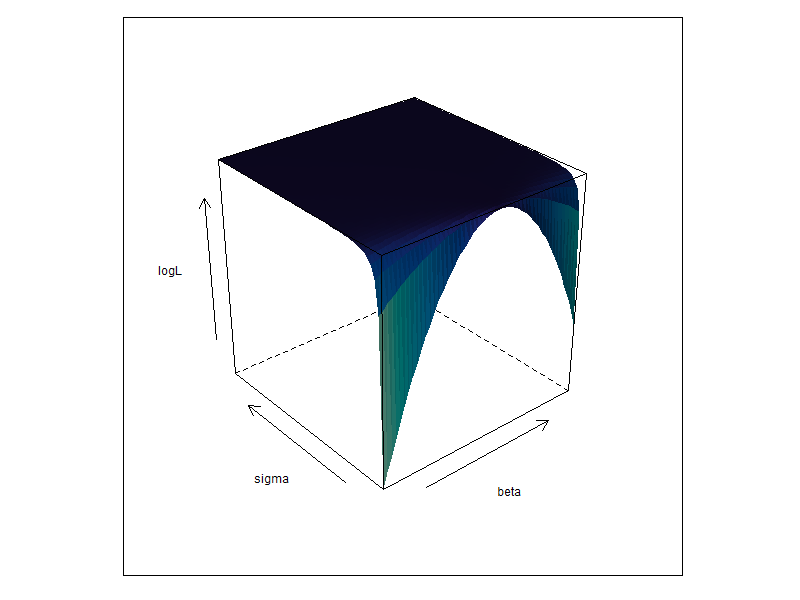
\includegraphics[width=0.5\textwidth]{plot.png}
	\item This function therefore produces an estimation of the parameters that specify this maximum point 
	
		\begin{table}[h]
		\centering
		\caption{BFGS results}
		\label{tab:estimates}
		\begin{tabular}{|c|c|}
			\hline
			\textbf{Parameter} & \textbf{Estimate} \\
			\hline
			\colorbox{yellow}{Intercept ($\alpha$)} & \colorbox{yellow}{0.1398324} \\
			\colorbox{yellow}{$\beta$} & \colorbox{yellow}{2.7265559} \\
			$\sigma$ & -1.4390716 \\
			$\sigma^2$ & 2.070927 \\
			\hline
		\end{tabular}
	\end{table}
	
	\item Then I compared the parameters created by my function with the results of the lm function
	\lstinputlisting[language=R, firstline=153, lastline=155]{PS1_KB_Final.R}
	
	
	
	
	\begin{table}[h]
		\centering
		\caption{OLS (lm) results}
		\label{tab:coefficients}
		\begin{tabular}{|c|c|c|c|c|}
			\hline
			\textbf{Variable} & \textbf{Estimate} & \textbf{Std. Error} & \textbf{t value} & \textbf{Pr(\textgreater|t|)} \\
			\hline
			\colorbox{yellow}{(Intercept)} & \colorbox{yellow}{0.13919} & 0.25276 & 0.551 & 0.582 \\
			\colorbox{yellow}{x($\beta$)} & \colorbox{yellow}{2.72670} & 0.04159 & 65.564 & $<2e-16$ \\
			\hline
		\end{tabular}
	\end{table}
	
	\item We can see in the highlighted terms that we are getting the same estimates for both the intercept ($\alpha$) and $\beta$ because both the BFGS algorithm and the OLS function are, in theory, consistent estimators of the true underlying parameter of interest 
		\begin{itemize}
			\item In this case, an on average effect of the covariate on the outcome
		\end{itemize}
	\item At some point the answers we get using the different methods would not be the same because they are different estimators
	\item For instance, OLS is closed form in the sense that we have the data and we plug it in to get estimates, while MLE is more complex as it uses numeric approximations
	\item So, in theory if we had a large amount of data, they will get closer to true estimate, but MLE is \textbf{not an unbiased estimator}
	
\end{itemize}


\end{document}
